\documentclass[tikz, border = 2pt]{standalone}

%---------------------------------------------------------------------------%
% PACKAGES                                                                  %
%---------------------------------------------------------------------------%

%----- MATH
%---------------------------------------------------------------------------%
\usepackage{amsmath, amssymb}

%----- FIGURES
%---------------------------------------------------------------------------%
\usepackage{pgfplots}
\pgfplotsset{compat=1.13}


\begin{document}

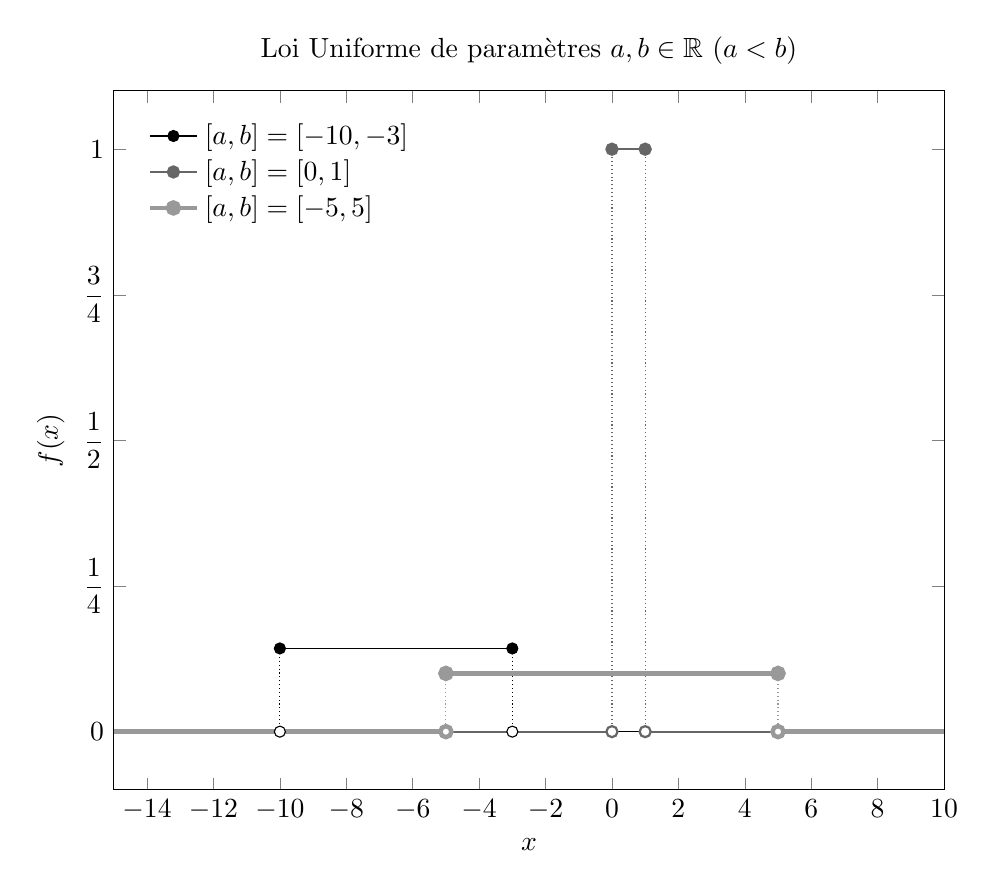
\begin{tikzpicture}
\begin{axis}[width = \textwidth,
title style = {align = center},
title={Loi Uniforme de param\`etres $a,b \in \mathbb{R}$ ($a<b$)},
xlabel={$x$},
ylabel={$f(x)$},
legend pos = north west,
legend style = {draw=none},
legend cell align = left,
xmin = -15,
xmax = 10,
ytick = {0,0.25,0.5,0.75,1},
yticklabels = {$0$, $\dfrac{1}{4}$, $\dfrac{1}{2}$, $\dfrac{3}{4}$, $1$},
ylabel near ticks
]
\draw[densely dotted] (-10,0) -- (-10,1/7);
\draw[densely dotted] (-3,0) -- (-3,1/7);
\draw[black!60, densely dotted] (0,0) -- (0,1);
\draw[black!60, densely dotted] (1,0) -- (1,1);
\draw[black!40, densely dotted] (-5,0) -- (-5,1/10);
\draw[black!40, densely dotted] (5,0) -- (5,1/10);
%
\addplot[black, samples = 2, domain = -15:-10, forget plot] {0};
\addplot[black, samples = 2, domain = -3:10, forget plot] {0};
\addplot[black, only marks, mark options = {fill = white}, forget plot] coordinates {(-10,0) (-3,0)};
\addplot[black, mark=*, samples = 2, domain = -10:-3] {1/7};
%
\addplot[black!60, thick, samples = 2, domain = -15:0, forget plot] {0};
\addplot[black!60, thick, samples = 2, domain = 1:10, forget plot] {0};
\addplot[black!60, only marks, mark options = {thick, fill = white}, forget plot] coordinates {(0,0) (1,0)};
\addplot[black!60, thick, mark=*, samples = 2, domain = 0:1] {1};
%
\addplot[black!40, ultra thick, samples = 2, domain = -15:-5, forget plot] {0};
\addplot[black!40, ultra thick, samples = 2, domain = 5:10, forget plot] {0};
\addplot[black!40, only marks, mark options = {ultra thick, fill = white}, forget plot] coordinates {(-5,0) (5,0)};
\addplot[black!40, ultra thick, mark=*, samples = 2, domain = -5:5] {1/10};
%
\legend{{$[a,b] = [-10,-3]$}, {$[a,b] = [0,1]$}, {$[a,b] = [-5,5]$}}
\end{axis}
\end{tikzpicture}

\end{document}